\documentclass[12pt, twoside]{book}
%\documentclass[12pt, oneside]{book}  % jednostranna tlac

%spravne nastavenie okrajov
\usepackage[a4paper,top=2.5cm,bottom=2.5cm,left=3.5cm,right=2cm]{geometry}
%zapnutie fontov pre UTF8 kodovanie
\usepackage[utf8]{inputenc}
\usepackage[T1]{fontenc}
%zapnutie slovenskeho delenia slov
%a automatickych nadpisov ako Obsah, Obrázok a pod. v slovencine
\usepackage[slovak]{babel} % vypnite pre prace v anglictine!

%nastavenie riadkovania podla smernice
\linespread{1.25} % hodnota 1.25 by mala zodpovedat 1.5 riadkovaniu

% balicek na vkladanie zdrojoveho kodu
\usepackage{listings}
% ukazky kodu su cislovane ako Listing 1,2,...
% tu je Listing zmenene na Algoritmus 1,2,...
\renewcommand{\lstlistingname}{Algoritmus}
% nastavenia balicka listings
% mozete pridat aj language=...
% na nastavenie najcastejsie pouzivaneho prog. jazyka
% takisto sa da zapnut cislovanie riadkov
\usepackage{color}
\lstloadlanguages{C,C++,csh,Java}

\lstdefinelanguage{TypeScript}{
  keywords={typeof, new, true, false, catch, function, return, null, 
catch, switch, var, if, in, while, do, else, case, break, let, number, boolean, string, any},
  keywordstyle=\color{blue}\bfseries,
  ndkeywords={class, export, boolean, throw, implements, import, this},
  ndkeywordstyle=\color{darkgray}\bfseries,
  identifierstyle=\color{black},
  sensitive=false,
  comment=[l]{//},
  morecomment=[s]{/*}{*/},
  commentstyle=\color{purple}\ttfamily,
  stringstyle=\color{red}\ttfamily,
  morestring=[b]',
  morestring=[b]"
}

\definecolor{red}{rgb}{0.6,0,0} 
\definecolor{blue}{rgb}{0,0,0.6}
\definecolor{green}{rgb}{0,0.8,0}
\definecolor{cyan}{rgb}{0.0,0.6,0.6}
\definecolor{darkblue}{rgb}{0.0,0.0,0.6}

\lstset{
language=csh,
basicstyle=\footnotesize\ttfamily,
numbers=left,
numberstyle=\tiny,
numbersep=5pt,
tabsize=2,
extendedchars=true,
breaklines=true,
frame=b,
stringstyle=\color{blue}\ttfamily,
showspaces=false,
showtabs=false,
xleftmargin=17pt,
framexleftmargin=17pt,
framexrightmargin=5pt,
framexbottommargin=4pt,
commentstyle=\color{green},
morecomment=[l]{//}, %use comment-line-style!
morecomment=[s]{/*}{*/}, %for multiline comments
showstringspaces=false,
emph={  async, await, 
var, abstract, event, new, struct,
as, explicit, null, switch,
base, extern, object, this,
bool, false, operator, throw,
break, finally, out, true,
byte, fixed, override, try,
case, float, params, typeof,
catch, for, private, uint,
char, foreach, protected, ulong,
checked, goto, public, unchecked,
class, if, readonly, unsafe,
const, implicit, ref, ushort,
continue, in, return, using,
decimal, int, sbyte, virtual,
default, interface, sealed, volatile,
delegate, internal, short, void,
do, is, sizeof, while,
double, lock, stackalloc,
else, long, static,
enum, namespace, string},
emphstyle={\color{cyan}\bfseries},
keywordstyle=\color{cyan},
identifierstyle=\color{red},
}

\lstdefinelanguage{XML}
{
  morestring=[b]",
  morestring=[s]{>}{<},
  morecomment=[s]{<?}{?>},
  stringstyle=\color{red},
  identifierstyle=\color{darkblue},
  keywordstyle=\color{cyan},
  morekeywords={xmlns,version,type}% list your attributes here
}


% balicek na vkladanie obrazkov
\usepackage{graphicx}
% balicek na vkladanie celych pdf dokumentov, tu zadanie
\usepackage{pdfpages}
% balicek na spravne formatovanie URL
\usepackage{url}
% balicek na hyperlinky v ramci dokumentu
% zrusime farebne ramiky okolo liniek aby pdf
% vyzeralo rovnako ako tlacena verzia
\usepackage[hidelinks,breaklinks]{hyperref}




% -------------------
% --- Definicia zakladnych pojmov
% --- Vyplnte podla vasho zadania, rok ma byt rok odovzdania
% -------------------
\def\mfrok{2023}
\def\mfnazov{Spracovanie dlhodobých meraní vybraných charakteristík Internetu}
\def\mftyp{Bakalárska práca}
\def\mfautor{Peter Trenčanský}
\def\mfskolitel{Ing. Dušan Bernát, PhD. }

%ak mate konzultanta, odkomentujte aj jeho meno na titulnom liste
\def\mfkonzultant{tit. Meno Priezvisko, tit. }  

\def\mfmiesto{Bratislava, \mfrok}

% študenti BIN a DAV odkomentujú príslušnú dvojicu riadkov
\def\mfodbor{ Informatika}
\def\program{ Informatika }
% pre BIN:
%\def\mfodbor{ Informatika a Biológia }
%\def\program{ Bioinformatika }
% pre DAV:
%\def\mfodbor{ Informatika a Matematika } 
%\def\program{ Dátová veda }

% Ak je školiteľ z FMFI, uvádzate katedru školiteľa, zrejme by mala byť aj na zadaní z AIS2
% Ak máte externého školiteľa, uvádzajte Katedru informatiky 
\def\mfpracovisko{ Katedra informatiky }

\begin{document}     
\frontmatter
\pagestyle{empty}

% -------------------
% --- Obalka ------
% -------------------

\begin{center}
\sc\large
Univerzita Komenského v Bratislave\\
Fakulta matematiky, fyziky a informatiky

\vfill

{\LARGE\mfnazov}\\
\mftyp
\end{center}

\vfill

{\sc\large 
\noindent \mfrok\\
\mfautor
}

\cleardoublepage
% --- koniec obalky ----

% -------------------
% --- Titulný list
% -------------------


\noindent

\begin{center}
\sc  
\large
Univerzita Komenského v Bratislave\\
Fakulta matematiky, fyziky a informatiky

\vfill

{\LARGE\mfnazov}\\
\mftyp
\end{center}

\vfill

\noindent
\begin{tabular}{ll}
Študijný program: & \program \\
Študijný odbor: & \mfodbor \\
Školiace pracovisko: & \mfpracovisko \\
Školiteľ: & \mfskolitel \\
% Konzultant: & \mfkonzultant \\
\end{tabular}

\vfill


\noindent \mfmiesto\\
\mfautor

\cleardoublepage
% --- Koniec titulnej strany


% -------------------
% --- Zadanie z AIS
% -------------------
% v tlačenej verzii s podpismi zainteresovaných osôb.
% v elektronickej verzii sa zverejňuje zadanie bez podpisov
% v pracach v angličtine anglické aj slovenské zadanie

\newpage 
\setcounter{page}{2}
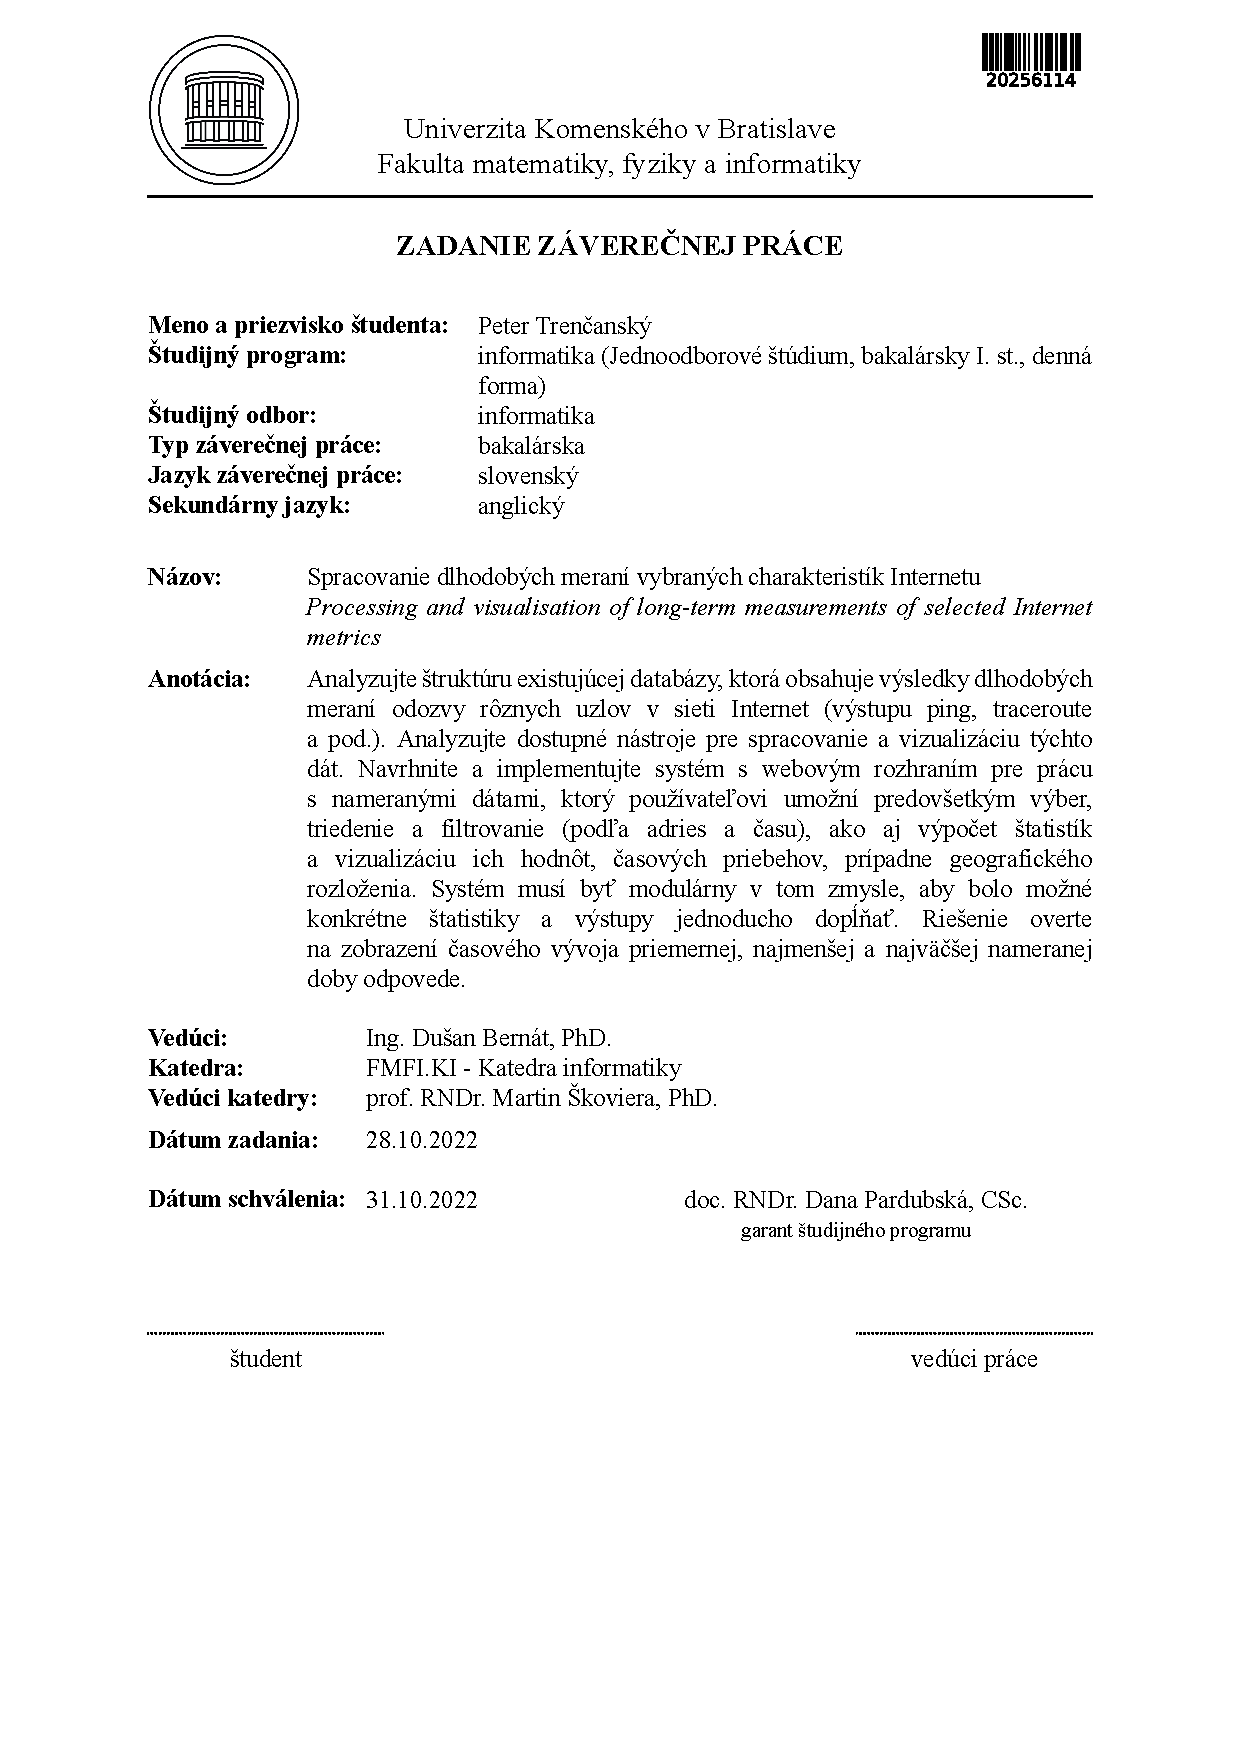
\includepdf{images/zadanie-zp_173220.pdf}

% --- Koniec zadania


% -------------------
%   Poďakovanie - nepovinné
% -------------------
\newpage 
\pagestyle{plain}
~

\vfill
{\bf Poďakovanie:} Chcel by som poďakovať môjmu školiteľovi, Ing. Dušanovi Bernátovi, PhD. za pomoca podporu pri tvorbe práce.

% --- Koniec poďakovania

% -------------------
%   Abstrakt - Slovensky
% -------------------
\newpage 
\section*{Abstrakt}


Táto bakalárska práca sa zaoberá spracovaním dlhodobých meraní vybraných charakteristík internetu. 
Cieľom práce je navrhnúť a implementovať systém s webovým rozhraním pre prácu s existujúcimi nameranými dátami. 
Systém by mal umožniť používateľovi výber, triedenie a filtrovanie dát podľa adries a času, ako aj výpočet štatistík a vizualizáciu ich hodnôt, 
časových priebehov a geografického rozloženia. 
Práca sa zaoberá možnosťami implementácie softvéru pre rôzne platformy a programovcie jazyky. Zaoberá sa tiež výberom databázového poskytovateľa a možnosťami vývoja frontendového a backendového riešenia.
Práca sa zaoberá aj testovaním aplikácie ručne aj automatizovane. 
Výsledkom práce je webová aplikácia, ktorá umožňuje vizualizovať výsledky meraní internetu v grafickej forme pomocou máp.
Tento systém by mal pomôcť používateľom lepšie pochopiť dlhodobé trendy a charakteristiky vývoja rýchlosti a dostupnosti internetu.

\paragraph*{Kľúčové slová:} internet, ping, vizualizácia, meranie, sklad
% --- Koniec Abstrakt - Slovensky


% -------------------
% --- Abstrakt - Anglicky 
% -------------------
\newpage 
\section*{Abstract}

This bachelor’s thesis deals with the processing of long-term measurements of selected characteristics of the internet. 
The aim of the thesis is to design and implement a system with a web interface for working with existing measured data. 
The system should allow the user to select, sort and filter data by addresses and time, as well as calculate statistics and 
visualize their values, time courses and geographical distribution. The thesis deals with the possibilities of implementing 
software for various platforms and programming languages. It also deals with the selection of a database provider and 
the possibilities for developing frontend and backend solution. 
Thesis also deals with testing of application both manually and automatically.
The result of the work is a web application that allows 
visualizing the results of internet measurements in graphic form using maps. This system should help users better understand 
long-term trends and characteristics of the development of internet speed and availability.

\paragraph*{Keywords:}  internet, ping, visualization, measurement, warehouse

% --- Koniec Abstrakt - Anglicky

% -------------------
% --- Predhovor - v informatike sa zvacsa nepouziva
% -------------------
%\newpage 
%
%\chapter*{Predhovor}
%
%Predhovor je všeobecná informácia o práci, obsahuje hlavnú charakteristiku práce 
%a okolnosti jej vzniku. Autor zdôvodní výber témy, stručne informuje o cieľoch 
%a význame práce, spomenie domáci a zahraničný kontext, komu je práca určená, 
%použité metódy, stav poznania; autor stručne charakterizuje svoj prístup a svoje 
%hľadisko. 
%
% --- Koniec Predhovor


% -------------------
% --- Obsah
% -------------------

\newpage 

\tableofcontents

% ---  Koniec Obsahu

% -------------------
% --- Zoznamy tabuliek, obrázkov - nepovinne
% -------------------

\newpage 

\listoffigures

% ---  Koniec Zoznamov

\mainmatter
\pagestyle{headings}


\input uvod.tex 

\input uvod_teoria.tex

\input navrh_riesenia.tex

\input moznosti_implementacie.tex

\input implementacia.tex

\input testovanie.tex

\input zaver.tex

% -------------------
% --- Bibliografia
% -------------------


\newpage	

\backmatter

\thispagestyle{empty}
\clearpage

\bibliographystyle{plain}
\bibliography{literatura} 

%Prípadne môžete napísať literatúru priamo tu
%\begin{thebibliography}{5}
 
%\bibitem{br1} MOLINA H. G. - ULLMAN J. D. - WIDOM J., 2002, Database Systems, Upper Saddle River : Prentice-Hall, 2002, 1119 s., Pearson International edition, 0-13-098043-9

%\bibitem{br2} MOLINA H. G. - ULLMAN J. D. - WIDOM J., 2000 , Databasse System implementation, New Jersey : Prentice-Hall, 2000, 653s., ???

%\bibitem{br3} ULLMAN J. D. - WIDOM J., 1997, A First Course in Database Systems, New Jersey : Prentice-Hall, 1997, 470s., 

%\bibitem{br4} PREFUSE, 2007, The Prefuse visualization toolkit,  [online] Dostupné na internete: <http://prefuse.org/>

%\bibitem{br5} PREFUSE Forum, Sourceforge - Prefuse Forum,  [online] Dostupné na internete: <http://sourceforge.net/projects/prefuse/>

%\end{thebibliography}

%---koniec Referencii

% -------------------
%--- Prilohy---
% -------------------

%Nepovinná časť prílohy obsahuje materiály, ktoré neboli zaradené priamo  do textu. Každá príloha sa začína na novej strane.
%Zoznam príloh je súčasťou obsahu.
%
\input appendixA.tex

\input appendixB.tex

\end{document}






